\documentclass{../lab}

\labacronym{MNO}
\labtitle{Nonlinear Spectroscopy and Magneto-Optics}

%\newcommand{\LabView}{http://dev-physicsadv.pantheon.berkeley.edu/node/119}
%\newcommand{\Physics111LibrarySite}{http://physics111.lib.berkeley.edu/Physics111/Reprints/MNO/MNO_index.html}
%\newcommand{\OpticsTutorial}{http://experimentationlab.berkeley.edu/OpticsTutorial}
%\newcommand{\DS345}{https://youtu.be/PrM8DHFOFS0}

\begin{document}

\maketitle

\tableofcontents

\section{Non-Linear Laser Spectroscopy and Magneto Optical Description (MNO)}

\begin{enumerate}
    \item \textbf{Note that there is NO eating or drinking in the 111-Lab anywhere, except in rooms 282 \& 286 LeConte on the bench with the BLUE stripe around it.} Thank You the Staff.

\end{enumerate}

This is an experiment on nonlinear laser spectroscopy and magneto-optics at the 111 Advanced Undergraduate Laboratory at Berkeley. The experiment consists of three parts. In the first part, students learn to operate a diode laser system and characterize its performance using a Fabry-Perot spectrum analyzer. In the second part, Doppler-broadened laser-induced fluorescence and Doppler-free saturated absorption spectra of the rubidium D2 line (780 nm) are recorded and analyzed. Finally, in the third part of the experiment, the near-resonant magneto-optical rotation is investigated. Nonlinear light-atom interaction leads to spectacular manifestations of the resonant Faraday effect - polarization plane rotation in a magnetic field applied along the direction of light propagation radically different from the linear case. In particular, narrow ($\sim$30 Hz) effective line widths are observed in this experiment corresponding to a rotation enhancement by some seven orders of magnitude compared to the linear Faraday rotation.

\begin{enumerate}
    \item Pre-requisites: OPT, Physics 137AB (137B may be taken concurrently)

    \item Days Allotted for the Experiment: 9

    \item Consecutive days: Yes

\end{enumerate}

\noindent\textbf{All pages in this lab. Note To print Full Lab Write-up click on each link below and print separately }

\begin{enumerate}
    \item \href{http://experimentationlab.berkeley.edu/node/119}{\textbf{}}\href{http://dev-physicsadv.pantheon.berkeley.edu/node/119}{\textbf{LabView}}\href{http://dev-physicsadv.pantheon.berkeley.edu/node/119}{\textbf{Program Descriptions}}

    \item \href{http://dev-physicsadv.pantheon.berkeley.edu/node/121#overlay-context=}{\textbf{Tuning the Laser}}
    
    \item \href{http://experimentationlab.berkeley.edu/node/80}{\textbf{Photodiode Circuit}}
\end{enumerate}

Reprints and reading materials can be found on the \href{http://physics111.lib.berkeley.edu/Physics111/Reprints/MNO/MNO\_index.html}{\textbf{Physics 111 Library Site}}

This lab will be graded 30\% on theory, 50\% on technique, and 20\% on analysis. For more information, see the \href{http://experimentationlab.berkeley.edu/syllabus}{\textbf{Advanced Lab Syllabus}}.

Comments: E-mail \href{\MailDonOrlando}{\textbf{Don Orlando}}

\emph{Acknowledgment and Disclaimer}. This material is based upon work supported by the National Science Foundation under Grant No. 9750873. ``Any opinions, findings and conclusions or recommendations expressed in this material are those of the author(s) and do not necessarily reflect the views of the National Science Foundation (NSF).''

\begin{center}
    \href{http://experimentationlab.berkeley.edu/sites/default/files/images/199px-Equipco_logo.png}{
\includegraphics[width=0.5\linewidth]{images/199px-Equipco_logo.png}}
\end{center}

Equipco Rentals of Concord, California donated two Newport Corporation, Research Series Optical Tables with Pneumatic Vibration Isolation mounts and table stands to our Physics Department. Equipco provides rentals, sales, and service of scientific instruments. Visit the \href{http://www.equipcoservices.com/}{\textbf{Equipco Environmental Equipment Rental Website}} for more information about their products or call direct at 1-888-234-5678 if you have a specific need. They have a wide selection of instruments available for donation to UC Berkeley.

\emph{Laser Restrictions.} The laser in this experiment beginning in Fall 2010 is a prototype being used in the development of an improved instructional experiment for the Physics 111 lab. The laser will not be distributed to another user. Installation and use of the laser in the experiment will be under the supervision of the U.C. Berkeley Laser Safety Officer to assure that personnel are properly trained and are not exposed to dangerous levels of radiation. This laser will be held by the U.C. Berkeley Physics Department for testing purposes, after which it will be destroyed.

D. Budker, D. Orlando, V. Yashchuk

\section{Magneto-Optics Photos}

\noindent
\href{http://dev-physicsadv.pantheon.berkeley.edu/sites/default/files/IMG\_4080.JPG}{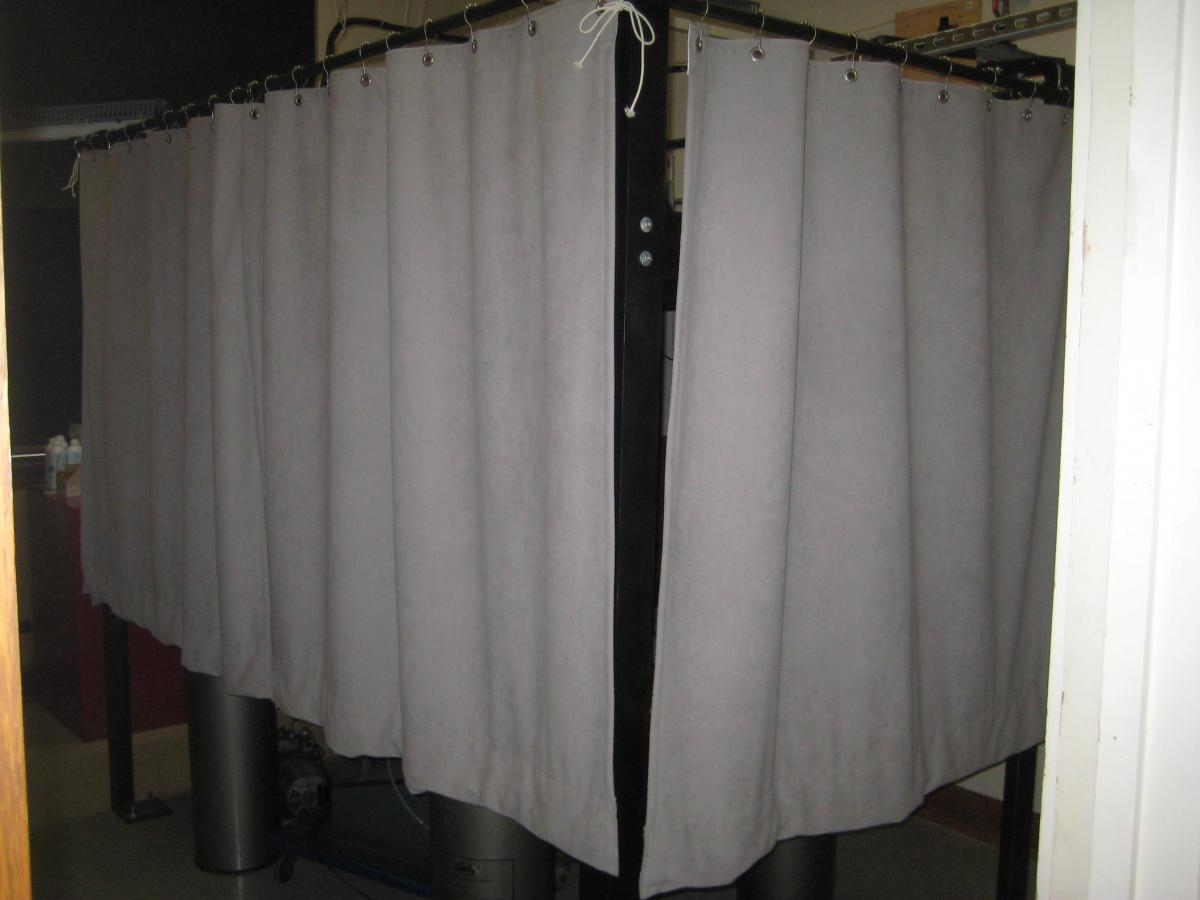
\includegraphics[width=0.33\linewidth]{images/IMG_4080.JPG}}
\href{http://dev-physicsadv.pantheon.berkeley.edu/sites/default/files/IMG\_4083.JPG}{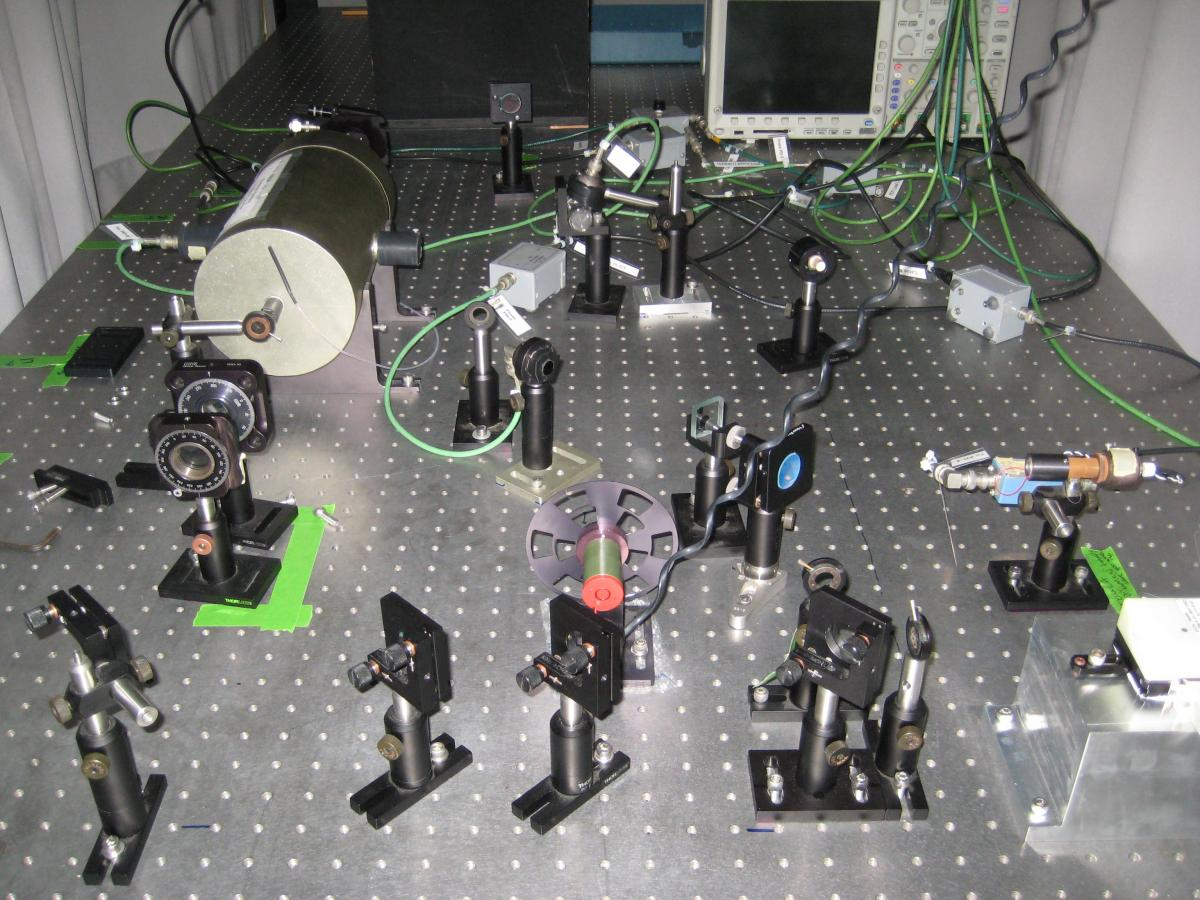
\includegraphics[width=0.33\linewidth]{images/IMG_4083.JPG}}
\href{http://dev-physicsadv.pantheon.berkeley.edu/sites/default/files/IMG\_4081.JPG}{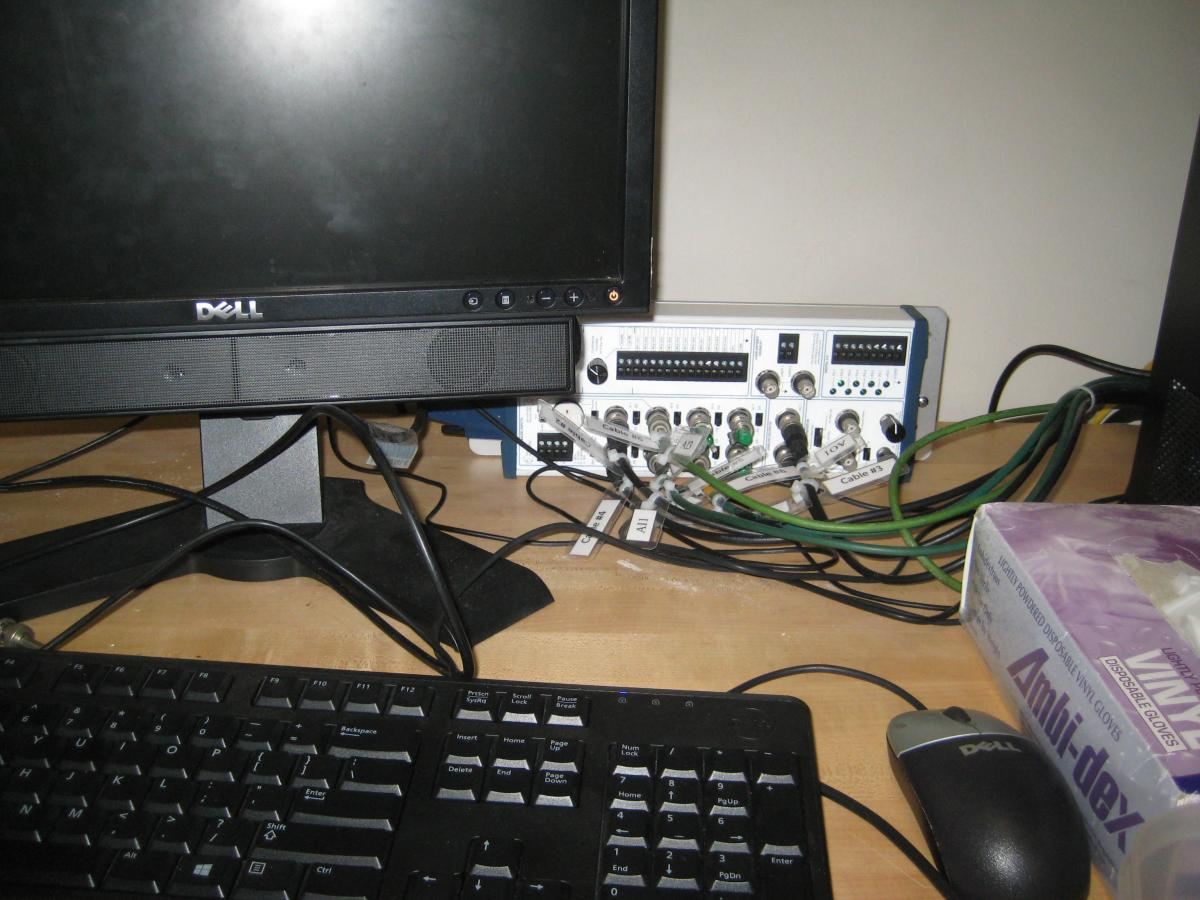
\includegraphics[width=0.33\linewidth]{images/IMG_4081.JPG}}

\noindent

\section{Before the 1st Day of Lab}
\label{sec:BeforeFirstDay}

\textbf{Complete the following before your experiment's scheduled start date:}

\begin{enumerate}
    \item View the two videos \href{http://youtu.be/JZJlyaIT3B4}{\textbf{Introduction, Part-1 video}} and the \href{http://youtu.be/h81p2LXkgZY}{\textbf{Introduction, Part-2 video}}.

    \item Before using the apparatus in this experiment, you must complete training in the safe use of lasers detailed on the \href{http://experimentationlab.berkeley.edu/lasersafety}{\textbf{Laser Safety Training}} page. This includes readings, watching a video, taking a quiz, and filling out a form.

    \item Complete the \href{http://experimentationlab.berkeley.edu/MNOprelab}{\textbf{MNO Pre Lab and Evaluation}} sheets. Print, fill it out and turn in your answers with the sheet. The Pre-Lab must be printed separately. Discuss the experiment and pre-lab questions with any faculty member or GSI and get it signed off by that faculty member or GSI. Turn in the signed pre-lab sheet with your lab report.

    \item View the optics tutorial, a review of the principles of optics, \href{http://experimentationlab.berkeley.edu/sites/default/files/ATM/fundamental-Optics.pdf}{\textbf{Fundamentals of Optics Tutorial}} and the \href{http://youtu.be/zUGBt5vc5FA}{\textbf{Optical Instruments Video}}, \href{http://youtu.be/wyBOVjU5bBQ}{\textbf{Energy Levels (part-1) Video}} and \href{http://youtu.be/Eypw0DmVBxk}{\textbf{Energy Levels (part-2) Video}}.

    \item Last day of the experiment please fill out the \href{\ExperimentEvaluation}{\textbf{Experiment Evaluation}}

\end{enumerate}

\noindent\textbf{Suggested Reading:}

\begin{enumerate}
    \item Technical description and instruction manual of the extended cavity diode laser: ECDL-7840R

    \item Fabry-Perot Spectrum Analyzers: ``Technical Memorandum on Fabry-Perot Interferometry''. Burleigh Instruments. Use this article to get some definitions and formulas. Most intermediate optics texts have a detailed analysis of how the fringes are formed, and a derivation of the transmission function

    \item Fabry-Perot Interferometer Instructions. ``\href{http://physics111.lib.berkeley.edu/Physics111/Reprints/MNO/Fabry-Perot\_Instructions\_OCR.pdf}{\textbf{Fabry-Perot Interferometer Instructions}}''. A guide to the use and settings of the FP Interferometer used in this experiment.

    \item D. W. Preston, ``\href{http://ajp.aapt.org/resource/1/ajpias/v64/i11/p1432\_s1}{\textbf{Doppler-free saturated absorption spectroscopy: Laser spectroscopy}}'', Am. J. Phys. 64(11), (1996). p. 1432-1436. (A fairly good introductory article (none better around).) \href{http://physics111.lib.berkeley.edu/Physics111/Reprints/MNO/03-Doppler\_Free\_Saturated\_Absoprtion.pdf}{\textbf{Searchable Page}}

    \item Saturation Spectroscopy: D. W. Preston and C. E. Wieman, ``\href{http://physics111.lib.berkeley.edu/Physics111/Reprints/MNO/04-Doppler\_Free\_Saturated\_Absoprtion.pdf}{\textbf{Doppler-free saturated absorption: laser spectroscopy}}''. An advanced laboratory write-up (09/1994; unpublished), p. 1-32. A more detailed version of the above.

    \item Diode Lasers: C. E. Wieman and L. Hollberg, ``\href{http://rsi.aip.org/resource/1/rsinak/v62/i1/p1\_s1}{\textbf{Using Diode Lasers for Atomic Physics}}'', Rev. Sci. Instrum. 62 (1), January 1991; p. 1-21. (A good article if you want to know how diode lasers work and how they are used.)

    \item D. Budker, D. J. Orlando, and V. Yashchuk, ``\href{http://ajp.aapt.org/resource/1/ajpias/v67/i7/p584\_s1}{\textbf{Nonlinear Laser Spectroscopy and Magneto-Optics}}'', Am. J. Phys. \textbf{67}, 584 (1999). (Covers the physics in the latter part of the lab.)

    \item Michael Lang. ``\href{http://physics111.lib.berkeley.edu/Physics111/Reprints/MNO/05-External\_Cavity\_Designs.pdf}{\textbf{External Cavity Designs Satisfy Stringent Demands}}''; Laser Focus World; June 1996, Pg. 1432-1436;

    \item T. J. Sumner, J. M. Pendlebury, and K. F. Smith ``\href{http://physics111.lib.berkeley.edu/Physics111/Reprints/MNO/06-Conventional\_Magnetic\_Shielding.pdf}{\textbf{Conventional Magnetic Shielding}}''; J. Physics D. Applied Physics 20 (1987) Pg. 1095-1101

    \item L. M. Barkov, D. A. Melik-Pashayev and M. S. Zolotorev ``\href{http://physics111.lib.berkeley.edu/Physics111/Reprints/MNO/08-Nonlinear\_Faraday\_Rotation.pdf}{\textbf{Non-Linear Faraday Rotation in Samarium Vapor}}''; Optics Communications Vol. 70, No. 6, 15 April 1989

    \item Dmirty Budker, Valeriy Yashchiek, and Max Zolotorev ``\href{http://physics111.lib.berkeley.edu/Physics111/Reprints/MNO/09-Resonant\_Magneto-Optical\_Rotation.pdf}{\textbf{Resonant Magneto-Optical Rotation: New Twists in an Old Plot}}''; Nuclear Science Division Dec 1997; LBNL-41149, UC-000 Preprint

    \item University of Florida, Department of Physics, Advanced Physics Lab, \href{http://www.phys.ufl.edu/courses/phy4803L/group\_III/sat\_absorbtion/SatAbs.pdf}{\textbf{Saturated Absorption Spectroscopy}}

    \item Information about the Lock-In Amplifier Used in this lab \href{http://physics111.lib.berkeley.edu/Physics111/Reprints/NMR/Lock-in-Amp.pdf}{\textbf{Lock-in Amp}},\href{http://physics111.lib.berkeley.edu/Physics111/Reprints/NMR/About-Lock-Ins.pdf}{\textbf{Lock-ins}}

\end{enumerate}

\noindent Other reprints and reference materials can be found on the \href{http://physics111.lib.berkeley.edu/Physics111/Reprints/MNO/MNO\_index.html}{\textbf{Physics 111 Library Site}}

You should keep a laboratory notebook. The notebook should contain a detailed record of everything that was done and how/why it was done, as well as all of the data and analysis, also with plenty of how/why entries. This will aid you when you write your report.

\section{Objectives}

\begin{itemize}
    \item Learn what real experimental physics is about

    \item Learn the synergy between experimental and theoretical work

    \item Learn to use pieces of equipment that are commonly used in research

    \item Learn how measurements are performed, analyzed, and interpreted.

    \item Learn how to present your work and results

    \item Learn problem solving strategies

    \item Learn how to manage and organize your time

\end{itemize}

\section{Note on the intent and scope of this laboratory manual}

This manual is intended to provide a general guidance for the lab. It is not designed to explain all the physics necessary for understanding this experiment, nor is it a ``cook-book'' telling you exactly which buttons to press, etc. It is up to the student to become familiar with the necessary material in the reprints, and to figure out the exact procedure necessary for completion of the assignments in the lab. Talk with an instructor often, but not until you have given the physics and procedures some thought first. We are here to instruct and help, but not to do your thinking for you.

\subsection{General}

\begin{enumerate}
    \item W. Demtroder. \emph{Laser Spectroscopy}. Springer, 1996.

    \item \href{http://experimentationlab.berkeley.edu/OpticsTutorial}{\textbf{Optics Tutorial}}

\end{enumerate}

\section{Note on Safety (please do not ignore)}

There are two major sources of danger in this experiment: laser radiation (780 nm, 45 mW continuous wave) and moderately high voltages present on some of the equipment (250 VDC at the scanning confocal Fabry-Perot (F-P) spectrum analyzer). The onset of permanent damage to the eye is at $>$5 mW. Any potential difference greater than 30 volts is potentially shocking. Please observe the following simple rules that will help you stay out of harm's way:

\begin{enumerate}
    \item When the laser is on, always wear the protective safety eyewear provided. The laser goggles available for this experiment absorb the infrared (IR) radiation from the laser and transmit visible light. Therefore, they will not hinder general visibility. While you are working on beam alignment you can use the blue night-vision viewer converting IR into visible light to see the laser beam without any danger. Please refer to Appendix IV about optics.

    \item A general rule for laser operators is to remove watches and jewelry because laser beams can get accidentally reflected in an uncontrolled fashion from watches or rings when a hand crosses the laser beam path.

    \item Make sure the curtains are closed when using the laser and before leaving.

    \item Do not look directly into the laser beam under any circumstances.

    \item This is the most important rule: always use common sense and think before doing anything.

\end{enumerate}

\section{Introduction}

The laser spectroscopy has been useful in a variety of applications throughout the years. It has been used in medicine, chemistry, material science, environmental research and many other fields. Combustion processes, atmospheric monitoring, water and vegetation surveillance, and medical diagnostics are but a few applications of the broader spectrum.

The ``Nonlinear Spectroscopy and Magneto-optics'' experiment is a good introduction to laser spectroscopy. The experiment itself will consist of three parts whose set up is fairly simple. In the first part you will learn a little about the diode laser and its operation. As you get familiar with the laser's operation, you will test the laser's performance using the Fabry-Perot spectrum analyzer. In the second part of the experiment you will record and analyze Doppler-broadened laser induced fluorescence and Doppler-free saturated absorption spectra of the rubidium. In the third part of the experiment we will investigate the near-resonant magneto-optical rotation. To get familiar with these concepts it is strongly recommended that you read the ``Nonlinear Laser Spectroscopy and Magneto-Optics'' article written by Dmitry Budker, Donald Orlando, and Valery Yashchuk. This article covers everything you need to know to complete this experiment. It is provided in the reprints for your convenience.

\section{Apparatus}

\textbf{If you can't find something, feel the equipment is faulty or needs to be aligned, or have any other issues of the sort, talk to Don. }

\textbf{*DO NOT TOUCH THE FOLLOWING KNOBS ON THE LASER CONTROLLER*}

\begin{enumerate}
    \item SWEEP KNOB

    \item SCAN KNOB

    \item OFFSET KNOB

    \item TEMPERATURE ADJUST

\end{enumerate}

In this lab we are going to use an ECDL-7840R Extended Cavity Diode Laser. This is a tunable, narrow line width (100 kHz) laser that has the capability of changing the wavelength range internally. Please be very gentle with this unit and do not turn any knobs unless instructed to do so. This laser system is very expensive! Do not touch the sweep or scan knobs on the laser unless absolutely necessary and never adjust the temperature without instructor assistance.

\begin{itemize}
    \item \textbf{Note:} There are overhead lights to help you see the equipment--the switch for the lights is located on the top rack near the door. At the end of each lab day, be sure to power off all equipment, turn off the overhead lights, and close the curtains on all sides to keep the station clean.

\end{itemize}

\subsection{ECDL-7840R Laser and Electronic Control Unit (ECU)}
\label{subsec:ECDL7840RLaser}

The ECDL-7840R Laser Input is connected to ECDL-7840R Electronic Control Unit (ECU) Laser Output. The ECU allows you to control the lasers' current input, wavelength, and temperature.The ECU is connected to the laser head via a gray cable. The 1:10 divider allows you to ``zoom in'' on your spectrum for finer detail. The 1:10 divider is a small brown box that should be located on the desk with the computer (put back when not in use) and has a ``$\div$10'' label.

The ECDL-7840R (Laser) changes wave length in three ways. First by adjusting the distance of an internal cavity in the laser head with a piezo electric device (PZT). Second, by varying the applied current to the diode itself and third by controlling the temperature of the diode. The temperature of the diode should not need to be adjusted, if you think you need to change the temperature talk to Don Orlando, though almost certainly temperature is not the problem. The ECU front panel is broken up into three sections, current, thermo, and PZT controls. The sweep knob (in the current section) sets the allowed current range when being scanned from some set center current. To set the center current the level knob is used. Note: the LCD current indicator does not keep up with the sweep rate so it is only useful to display the center current, this means it is possible to sweep above the current limit without the indicator displaying this, please monitor the current limit LED instead. The PZT control section is similar to the current section. The scan knob changes the range that the PZT is scanned over and the offset changes the center wavelength the PZT scans. On the back of the ECU there is an EXT input (labeled PZT input) that is used to connect the ECU to the computer or signal generator. Once connected, the computer/signal generator can adjust the current/PZT. There is an INT/EXT switch that switches from the external source to an internal 30 Hz triangle wave. This switch should be set to EXT for the entire experiment.

\subsection{Optical Setup}

The optical set up for this experiment is fairly simple. The laser beam coming from the ECDL-7840R LASER passes through a Diaphragm Iris and is split into several beams so that we can set up all three parts of the experiment using one beam at all times. The splitting of the beam is done using the beam splitters. The beam splitters in our lab are just pieces of microscopic cover glass attached to the adjustable mirror mounts. The optical set up for this experiment is shown in the Figure \ref{fig:DiagramOfOpticalSetup}. As you read this section, refer to both the diagram in Figure \ref{fig:DiagramOfOpticalSetup} and also the actual optical set up on the table. Keep in mind that as you follow the actual setup, you must be careful not to touch anything. Even slightest movement of the mirrors, beam splitters and other parts will result in misalignment of the experiment not to mention that you will leave fingerprints all over the mirrors and beam splitters. If that happens, you will create more tedious work for yourself and others trying to align the components.

The first beam splitter (BS-1 as labeled in Figure \ref{fig:DiagramOfOpticalSetup}) is used to split the incoming laser beam into two beams. One of the beams will be used for the Fabry-Perot spectrum analyzer. The other beam will be split by BS-2 and BS-3 to be used in Laser induced fluorescence and Doppler-free saturation spectroscopy. Finally, the laser beam coming out of BS-3 will be split again by BS-4 for the magneto-optical part of the experiment. The optical setup of each individual part of the experiment will be discussed in greater detail in the procedure section. Roughly speaking, the laser beam coming out of the BS-1 for the Fabry-Perot part of the experiment passes through the Diaphragm Iris and goes into the Fabry-Perot spectrum analyzer. The output of the spectrum analyzer is connected to the photodiode sensor (PD-4). The laser beam coming from BS-2 for the laser-induced fluorescence and Doppler-free saturation spectroscopy part of the experiment passes through the optical chopper and then through the center of a Rubidium cell. A second beam coming from BS-3 is reflected by a mirror, M1 as shown in Figure \ref{fig:DiagramOfOpticalSetup}. The reflected beam also passes through the rubidium cell but in the opposite direction. This beam is then reflected by another mirror, M2, and is sent to a photodiode sensor, PD-3. Another photodiode sensor, PD-5 is placed next to a rubidium cell as shown in Figure \ref{fig:DiagramOfOpticalSetup}. Finally, in the magneto-optical part of the experiment, the laser beam coming from BS-4 is passed through two polarizers. It is then passed through another rubidium cell that is placed inside magnetic coils (the cell with coils is shielded). The laser beam exits the rubidium cell and enters the polarimeter (PBS) that splits the beam into two. The two beams enter two photodiode sensors, PD-1 and PD-2. On the side of the shielded cell with coils is located another photodiode, PD-6.

\begin{figure}[h]
    \centering
    \href{http://experimentationlab.berkeley.edu/sites/default/files/images/MNOimage003.gif}{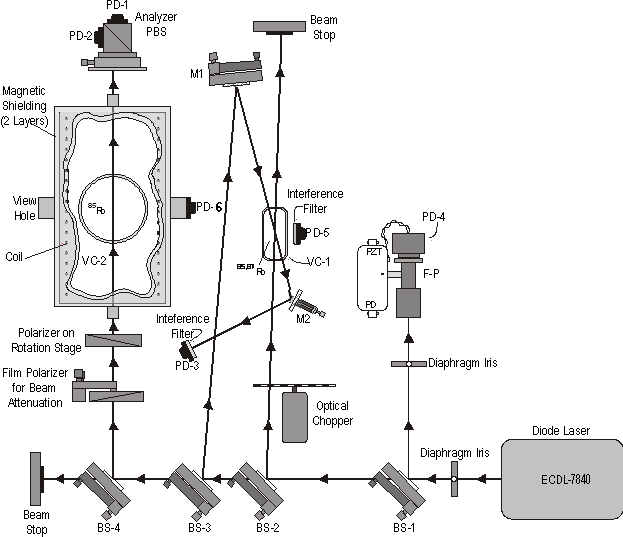
\includegraphics[width=0.6\linewidth]{images/MNOimage003.png}}
    \caption{Diagram of the optical set-up}
    \label{fig:DiagramOfOpticalSetup}
\end{figure}

\subsection{Photodiode circuit}

In this lab, we use several silicon photodiodes to measure the intensity of laser beams and of atomic fluorescence light. The simple circuitry that we use (the photodiode bias and load resistor box) is shown in Figure \ref{fig:SchematicOfPhotodiodeBiasAndLoadResistorBox}. Here, the photodiode operates in the \emph{photoconductive} mode in which a reverse bias is applied to the diode and no current is flowing through the circuit in the absence of light (neglecting the \emph{dark} current, which actually becomes important in small-signal applications). In the absence of current, there is also no output voltage across the load resistor. When a photon strikes the photodiode, it creates an electron-hole pair in the conductivity band in the carrier-depleted zone of the photodiode's pn-junction. The \emph{quantum efficiency} of this process may reach nearly 100\%, meaning that there is one pair produced per incident photon. The charges then flow through the load resistor upon the action of the bias voltage, thus producing output voltage.

\begin{figure}[h]
    \centering
    \href{http://experimentationlab.berkeley.edu/sites/default/files/images/MNOimage023.gif}{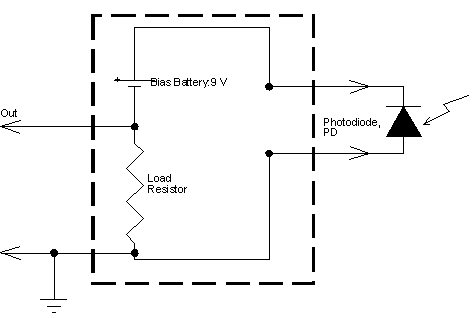
\includegraphics[width=0.6\linewidth]{images/MNOimage023.png}}
    \caption{Schematic of the photodiode bias and load resistor box. \href{http://experimentationlab.berkeley.edu/sites/default/files/images/PhotoDiode-10DP.pdf}{\textbf{PhotoDiode-10DP data Sheet}}}
    \label{fig:SchematicOfPhotodiodeBiasAndLoadResistorBox}
\end{figure}

All six photodiode sensors are connected to photodiode load resistors. The PD-5 used in the Diode Scan section of the lab is connected to a 1M$\Omega$ PD Load Resistor. The output of that load resistor is then connected to AI 2 input of the NI BNC 2120 Breakout Box (located behind the computer screen, you should be familiar with this DAQ box from 111a). The BNC 2120 Breakout Box is used to input BNC cable data to the DAQ card installed in the computer. See the diagram of the electrical connections in Figure \ref{fig:BlockDiagramOfElectricalConnections} and list of connections in Table \ref{table:ListOfConnectionsInvolvingDAQ}. Figure \ref{fig:BlockDiagramOfElectricalConnections} shows the connections for the Diode Scan part of the experiment and B-Field scan, although all connections are not used for both parts.

Referring to Figure \ref{fig:BlockDiagramOfElectricalConnections}, you can see that the PD-4 is connected to the 100K$\Omega$ Load Resistor whose output is connected to AI 0 of the Breakout Box. The PD-3 is also connected to 1M$\Omega$ Load Resistor whose output will be connected at some point of the experiment to SR830 DSP Lock-In amplifier (do not connect the PD Load resistor to the Lock-in yet). Lock-in amplifiers are used to detect and measure very small AC signals. Accurate measurements can be made even when the small signal is obscured by noise sources. Lock in amplifiers use a technique known as phase-sensitive detection to single out the component of the signal at a specific reference frequency and phase. Noise frequencies other than the reference frequency are rejected and do not affect the measurement. In our experiment we will connect Channel 1 Output of the Lock-in to the AI 1 Input of the Breakout Box via Cable 2. (The switch for the lock-in amplifier is in the back of the unit). The Ref In of the Lock-in is connected to the SR 540 Chopper Controller's ``f''/f diff Input. The SR 540 Chopper Controller controls the optical chopper that chops the laser beam coming from BS-2. The PD-2 is connected to the 100k$\Omega$ Load resistor whose output goes to AI 4 of the Breakout Box. The PD-1 is also connected to the 100k$\Omega$ Load Resistor whose output is connected to AI 3 of the Breakout Box.

In the Diode Scan section of the lab, the AO 0 of the Breakout box should be directly connected to the Input of the ECDL-7840R. When doing the B-Field Scan, the AO 1 should be connected to the magnetic coils in either of the two ways. One way is to connected it through a 2.5 k$\Omega$ Load Resistor (Little Blue Box). Second way (\textbf{Highly recommended}) is to connect it to Input 1 of the COIL DRVER via Cable 3. The COIL DRIVER is located on the rack above the magnetic coils (shielded metal chamber). The COIL DRIVER OUTPUT 1 should be connected to the magnetic coils. The apparatus is already setup for the second way, and you shouldn't need to change it. The Monitor 1 input of the Coil Driver should be monitored by a DMM. The 2.5 k$\Omega$ resistor is there so that you can also ``zoom-in'' on your spectrum for better detail. A chart of the connections from the DAQ is below in Table \ref{table:ListOfConnectionsInvolvingDAQ}. The cable numbers are on a label on each cable.

\begin{table}[h]
    \centering
    \href{http://experimentationlab.berkeley.edu/sites/default/files/images/350px-Connectionchart.jpg}{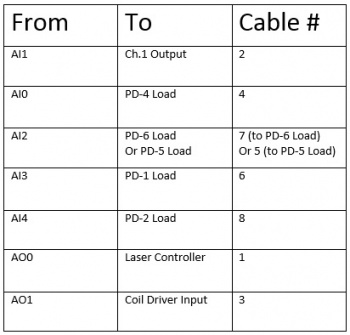
\includegraphics[width=0.5\linewidth]{images/350px-Connectionchart.jpg}}
    \caption{List of connections involving the DAQ}
    \label{table:ListOfConnectionsInvolvingDAQ}
\end{table}

\begin{figure}[h]
    \centering
    \href{http://experimentationlab.berkeley.edu/sites/default/files/images/MNOfigure2.jpg}{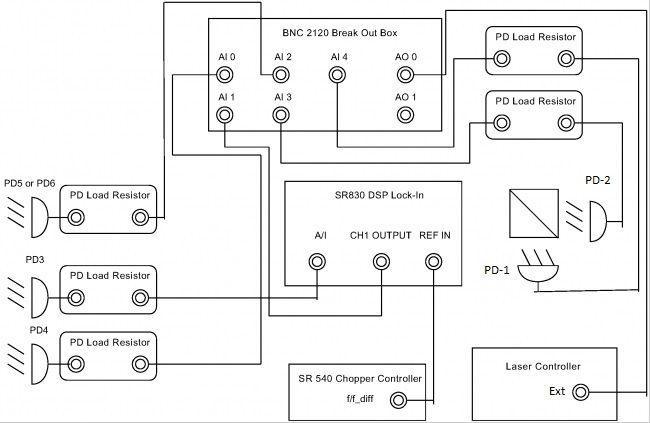
\includegraphics[width=0.5\linewidth]{images/MNOfigure2.jpg}}
    \caption{Block Diagram of the electrical connections for the Diode Scan part.}
    \label{fig:BlockDiagramOfElectricalConnections}
\end{figure}

\section{Procedure}

\subsection{Part 1: Laser Operation, Spectrum Analyzer}

In this part, you will learn to operate the diode laser, familiarize yourself with various parameters of the laser output, and learn to use the scanning confocal Fabry-Perot interferometer. Prior to turning on any of the equipment or changing any of the electrical connections, you should carefully read the relevant operating instructions and watch the videotape. Keep in mind you are dealing with expensive equipment ($\sim$\$7-8 thousand dollars for just the laser).

\subsubsection{Operating the Laser}
\label{subsubsec:OperatingTheLaser}

\begin{enumerate}
    \item Use the laser manual and the diagrams provided in the manual to identify all parts of the laser system: laser head (where the laser actually is), electronic control unit (ECU), wavelength control knobs on the laser (tuning knobs), laser output port. Read about the controls and indicators (see Section \hyperref[subsec:ECDL7840RLaser]{ECDL-7840R Laser and Electronic Control Unit (ECU)} for a quick overview or see the \href{http://physics111.lib.berkeley.edu/Physics111/Equipment\_Manuals/manual\_D1\_ECDL\_laser.pdf}{\textbf{Technical description and instruction manual of the extended cavity diode laser: ECDL-7840R}} for a more in depth explanation)on the ECU.

    \item To get the ECU and ECDL-7840R Laser ready for operation, follow the following steps:
    \begin{itemize}
        \item Reset all the knobs on the front panel by turning them all the way to the left (counterclockwise), except for the level knob which just keeps turning. For your convenience, you may want to put markers on them to keep track of their positions (see image below--we used green tape as the markers).
        \begin{center}
            \href{http://dev-physicsadv.pantheon.berkeley.edu/sites/default/files/MNO_pics/800px-ECUknobs.jpg}{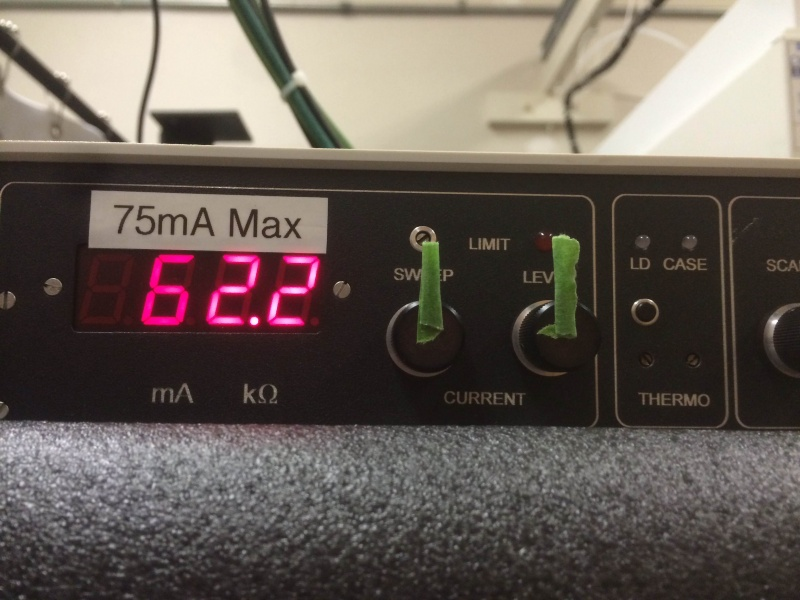
\includegraphics[width=0.5\linewidth]{images/800px-ECUknobs.jpg}}
        \end{center}
        
        \item Make the following adjustments:
    
        \begin{itemize}
            \item Sweep knob: Turn 130 degrees to the right (clockwise).
    
            \item Level knob: Set the level to about 62.3 mA.
    
            \item Scan knob: Turn all the way to the right.
    
            \item Offset knob: Turn 8 turns to the right, and then an additional 45 degrees (approximately) to the right.
        \end{itemize}

        \item After you have made the adjustments, you should see a faint glow in the glass Rb chamber using the Blue Night Vision Viewer (press the red button while looking through the Viewer, and adjust to the focus to see clearly). If you do not see a glow using the Viewer, trying adjusting the Offset knob slightly either way until you see it. Be careful not to turn the knob too far, for this will throw off your other measurements.
    \end{itemize}
    
    \item Make sure you know where the beam will go before you turn on the laser.

    \item Check all connections between the laser system and other components shown in Figure \ref{fig:DiagramOfOpticalSetup} and Figure \ref{fig:BlockDiagramOfElectricalConnections}. They should all be in place, but check them anyway. Again, be careful not to touch the optical instruments. It is very difficult to line up the optics! Locate the experiment setup Figure \ref{fig:DiagramOfOpticalSetup} and print it out to follow the beam path.
    
    \item \textbf{Put on your safety goggles} and turn on the laser system. There is a on/off switch on the back of the ECU. Then to start operating the laser, hit the red switch on the right end of the ECU front panel with initials ``LD'' labeled beneath. The system should be left on all the time, even while the laser itself is not operating. On the left side of the ECU the current is displayed. Laser power is approximately proportional to (\emph{I}-\emph{I}thr), where \emph{I}thr$\approx$31 mAis the lasing threshold current.
    
    \item Now check for stray beams: If you do this experiment on consecutive days then check the beam path at the start of this experiment. If another group has used the laser since you're been operating the laser then you should re-check for stray beams when you turn on the laser. You should perform the survey of the laser beam paths to check if there are any stray beams (diffuse or specular) emanating from any part of the laser and its optics, and then document this in the laser log book in the wall pocket near the experiment.
    
    \item Checking for stray beams is done by using the IR Viewer and a white piece of paper or business card. If the IR Viewer is not in the room, ask a staff person to locate it. The IR viewer is blue in color and you use it with your goggles on. Using the paper card follow all of the beam paths through the Magneto Optical setup section (see Figure \ref{fig:DiagramOfOpticalSetup}). Note if the beam strays from its intended path. It should go through the lenses, beam splitters, and reflect from mirrors, but should NOT hit or reflect off of anything else (including the mounts) on the optical table. This laser beam is hazardous to your eyes if they are unprotected as you cannot see the laser light. Keep the goggles on at all times for your safety.
    
    \item To view the beams during the experiment (goggles on) use the IR visualization card, or the night vision viewer and a piece of paper. You can observe where the beam is going without actually blocking it by using a piece of \emph{lens paper} and the night vision viewer. This is especially helpful around mirrors or other tight spots.
    
    \textbf{Q.} What is the shape and size of the laser beam? Why is it elongated in one direction? By observing the beam size at different distances from the laser, roughly estimate the angular divergence of the beam. Is it close to being diffraction limited (meaning the minimum divergence with a given beam cross-section, sine theta $\sim$ wavelength/beam diameter?

    As shown on the diagram of the optical set-up (Figure \ref{fig:DiagramOfOpticalSetup}), small fractions of the laser beam are split with beam splitters mounted on adjustable mirror mounts. The first beam splitter directs laser light through a scanning confocal Fabry-Perot interferometer. Reprints for this lab contain a technical memo on Fabry-Perot interferometry written by Burleigh Instruments - a commercial manufacturer of F-P spectrum analyzers. In this experiment, we use a homemade F-P.
    
    In this lab, the FP serves two purposes. The first is as a frequency marker, so we know how far apart the peaks are when we take a spectrum. For reference, the peaks on the FP spectrum are spaced 1.50 GHz apart. The second is to see how well the laser is working. If the peaks are periodic, then the laser is working well, but if the peaks are absent or scattered around, that means either the laser is ``mode hopping'' or the FP is not aligned correctly. Also, make sure that you are not driving the FP with the signal generator. This causes the cavity length to oscillate and would produce irregular scans. You may accidentally be doing this if the signal generator is on and the cable labeled ``FP PZT Input'' connects the FP PZT and the high voltage amplifier. (\emph{This is confusing, there are two PZTs, one connected to the FP and one inside the laser. The one connected to the FP is used only for aligning the FP and if the cable FP PZT Input is plugged into the FP, unplug it now. \textbf{ Be sure not to accidentally turn the FP though, it is not very secure.}})
    
    \item In order to observe the transmission pattern of the F-P analyzer, check to see that the appropriate connections are made. Everything should be already there, but check it anyway. As shown on the diagram in Figure \ref{fig:BlockDiagramOfElectricalConnections}, the photodiode (PD-4) output of the F-P analyzer is connected to a photodiode 100 k$ \Omega $ Load resistor. (The circuit is described in \href{http://dev-physicsadv.pantheon.berkeley.edu/node/120}{\textbf{Photodiode Circuit}}). The output of the PD Load resistor is connected to the AI 0 input channel of the DAQ board (the BREAKOUT BOX). Connect the AO 0 from the Breakout Box to the Ext on the back of the ECU. The BNC cable from AO 1 can be left disconnected. Make sure the laser beam passes straight through the F-P spectrum analyzer. If it does not, you need to align it using the night vision viewer or the IR card. Be very gentle when aligning the optical instruments. When aligning the optics, use Figure \ref{fig:DiagramOfOpticalSetup} as your guide. Make sure you understand where the laser beams must enter and exit.
    
    In this lab, the experiment control and data acquisition are performed using a PC computer equipped with data acquisition and control card (DAQ). Input to and output from the card are accomplished through a BNC breakout box. The process is controlled by a LABVIEWTM program ``Diode Scan for 111 lab.vi''. A description of this program is given in\href{http://dev-physicsadv.pantheon.berkeley.edu/node/119}{\textbf{}}\href{http://dev-physicsadv.pantheon.berkeley.edu/node/119}{\textbf{LabView}} Program Descriptions, and a shortcut to it can be found on the DESKTOP of the computer dedicated to this experiment called MNO v2.llb.
    
    \item Set up the ``Diode Scan for 111 lab.vi'' program to do a 2Vpp scan and obtain the transmission spectrum of the F-P analyzer. \textbf{DO NOT exceed a range of $\pm$ 1.5V when scanning the PZT}. You should refer to\href{http://dev-physicsadv.pantheon.berkeley.edu/node/119}{\textbf{}}\href{http://dev-physicsadv.pantheon.berkeley.edu/node/119}{\textbf{LabView}} Program Descriptions for information on all the buttons and what they do. To start with you can use 1000 points per scan, 50 acquisitions per scan point, 500 points per sec acquisition rate, and -1.5V minimum. If you want to scan faster you can increase the acquisitions/sec or decrease the number of data points, either in a scan or per voltage. Some settings cause aliasing or change the voltage amplitude from the diode. What can you say about the laser mode structure based on your result?

\end{enumerate}

\subsubsection{Aligning the Fabry-Perot Interferometer}

\textbf{Do not do this section unless you are absolutely sure that the Fabry-Perot Interferometer needs to be aligned aka ask a staff member.}

This section should be only used when all other things have failed to fix the problem (i.e. the laser beam is aligned, you have the proper connections and etc.). Before you start aligning the Fabry-Perot Interferometer, talk with the staff members and explain why you think the F-P Interferometer needs to be aligned. Please refer to the \href{http://experimentationlab.berkeley.edu/OpticsTutorial}{\textbf{Optics Tutorial}}.

Instead of varying the frequency of the laser and observing the F-P spikes on Labview, you can use a signal generator to apply a changing voltage to the PZT in the interferometer while keeping the laser at a fixed frequency. This changes the length of the resonant cavity periodically. You can then make the necessary adjustments and watch the shape and of the F-P spikes change on the scope.

\begin{enumerate}
    \item Connect the output of the high voltage amplifier to the PZT on the Fabry-Perot interferometer.

    \item Connect the Wavetek signal generator or \href{https://youtu.be/PrM8DHFOFS0}{\textbf{DS 345}} output to the input of the high voltage amplifier and to the scope.

    \item Connect the output of the Fabry-Perot interferometer diode (the cable that normally goes from the Fabry-Perot through the variable resistor box to AI 0) to the other channel on the scope. (There is a cable with an coupler on the experimental table to use for this part).

    \item Set the Wavetek to a 100 Hz triangle wave and look at both channels on the scope at the same time.

    \item Adjust the amplitude of the Wavetek or \href{https://youtu.be/PrM8DHFOFS0}{\textbf{\textbf{DS 345}}} then  the output offset on the high voltage amplifier until the Fabry-Perot spikes are not overlapping.

    \item Adjust the time scale on the scope so that only 1 or 2 Fabry-Perot spikes are displayed.

    \item Adjust the alignment of the beam splitter, the size of the aperture, and the height of the Fabry-Perot interferometer so that the Fabry-Perot spikes are as large as possible and as symmetric as possible. Please refer to the \href{http://experimentationlab.berkeley.edu/OpticsTutorial}{\textbf{Optics Tutorial}}.

    \item If the peaks are still irregular, you may have to change the temperature of the laser by half a degree or so. Do not change the temperature yourself. Call for assistance from Don or an instructor.

\end{enumerate}

\textbf{Try not to adjust BS1 while aligning the interferometer. It will change the alignment of the other modules of the experiment, which are very sensitive.}

\subsubsection{Determining the Voltage to Frequency Conversion Factor}

The wavelength of the laser is set at 780nm $\pm$ 2nm. However 0.1 nm corresponds to $3 \times 10^{18}$ Hz and the frequency intervals we are interested in are on the order of 100 MHz. However the 1.5 GHz frequency markers from the FP \textbf{combined} with knowledge of the laser control voltage difference between two peaks allow you to derive a conversion between laser control voltage (which LabView records) and laser frequency.

Once the F-P interferometer is aligned and the laser is working correctly, take a scan over a frequency range that will sweep through a number of FP markers (a 2 V p-p scan should be sufficient). Save the scan to file then open and plot the data in Matlab or other programs you prefer. Calculate the voltage spacing between successive FP peaks to get a feel for how the laser's frequency changes with voltage.

The laser's frequency as a function of control voltage may not be a perfectly linear relationship. It should be sufficient to average these voltage intervals to come up with a conversion factor in units of Volts per 1.5 GHz which can be inverted to convert to the desired units of GHz/V. If this linear approximation of frequency as a function of voltage is not accurate enough, one can derive a quadratic expression for frequency as a function of voltage, however this is probably unnecessary.

\textbf{Important: When using the 1:10 zoom resistor the voltage to frequency conversion factor is different. To determine the new conversion factor repeat the process above with the zoom resistor connected. With the resistor you will need to scan at least 5 V p-p in order to fit two FP spikes on one scan.} Note: The zoom resistor may not be necessary with the new daq cards (as of summer 2013), try zooming in with the scan settings.

\section{How to tune the laser}

It is not likely the laser needs to be tuned by any means other than adjusting the current, especially if you followed the directions in step 2 of the \hyperref[subsubsec:OperatingTheLaser]{Operating the Laser} section. If the D2 line does not resonate at the 63.3 mA setting (if you are not able to see any glow in the glass Rb chamber using the blue IR night vision viewer), you may need to tune the laser. To do so, set the laser current to 63.3 mA. While using the night vision viewer, VERY SLOWLY turn the OFFSET knob on the laser until you see some light beams flicker in the 87/85 cell. Due to the behavior of the laser, this may only happen if you pass the point in one direction, but not the other. Since this knob is such a course adjustment, the flicker means you went through all the peaks really quickly. Try to leave the knob on a position so that you can see a constant glow in the tube. It doesn't matter which peak you are on, but some are brighter than others.

\subsection{Part 2: Tuning the laser to resonance, laser-induced fluorescence spectra}

In this part of the lab, you will tune the laser to the rubidium D2 resonance ($^2S_{1/2} \rightarrow {}^2P_{3/2}$)  at 780.2 nm and observe laser-induced fluorescence as the laser frequency is scanned across the atomic resonance. To do this, simply turn the LEVEL knob to 63.3 mA. This corresponds to 780.2 nm from the ECDL-7840. You can tell you have found the D2 resonance line by observing the 87/85 cell through the night vision viewer. When you are on resonance you will be able to see the path of the laser glow: this is the rubidium fluorescence.

\begin{itemize}
    \item Our goal now is to observe laser-induced fluorescence from Rb atoms in a vapor. Looking at the diagram in Figure \ref{fig:DiagramOfOpticalSetup}, we are going to use the laser beam that has passed through beam splitter BS-1. The following is already set up on the optical table and all you need is to check that everything is in place. Please refer to the \href{http://experimentationlab.berkeley.edu/OpticsTutorial}{\textbf{Optics Tutorial}}\. Do not dismount any of the components from the table and try to avoid touching the optical instruments unless you are in the process of aligning the beam.

\end{itemize}

\emph{Description of Beam Path:} The laser beam coming from BS-1 should pass through a beam splitter BS-2 that splits the beam into two. One of the beams passes through, and the other splits off at somewhere less than 90 degree angle towards an optical chopper. Passing through the optical chopper, the beam enters and exits the glass rubidium cell/chamber (the one outside the magnetic shield). The cell mounting and BS-2 can both be adjusted if necessary (Do not unless you are sure it is not aligned! In general, be careful not to touch or change the positions of the optical equipment because it is difficult to realign.) As indicated on the diagram, there should be a photodiode PD-5 placed facing the glass Rb cell. This photodiode has a 780 nm interference filter attached to the front side of the diode to reduce pick-up from room lights. The output of the photodiode is connected to the 1 M$\Omega$ Load resistor input. The output of the PD Load resistor is connected to the AI 2 input of the DAQ BNC connector box (the Breakout Box) via cable 5. The second beam that passes through the BS-2 is split in to two once again by a beam splitter BS-3. One of the beams passes right trough the BS-3 and the other is reflected off of it. The reflected beam is then sent to a mirror M1 where it is reflected to pass through the rubidium cell, but in the opposite direction. This beam exits the rubidium cell and is reflected once more by another mirror, M2. Finally this beam enters a photodiode sensor PD-3. The output of the PD-3 is connected to the PD Load Resistor. At this time, nothing is connected to the output of this load resistor, but in the next section you will connect it to the Lock in Amplifier. Connect the AO 0 from the Breakout Box to the BNC connection marked PZT on the back of the laser controller via Cable 1. Connect the AO 1 of the Breakout Box to the Input of the Coil Driver via cable 3. Start the Diode Scan LabView program using -1.5 V minimum, 3 V p-p, 1000 pts/scan, 50 acquisitions/pt, and 500 acquisitions/sec. If you do not see the correct signal in the diode scan program, redo step 2 listed in the \hyperref[subsubsec:OperatingTheLaser]{Operating the Laser} section. If you still don't see results, then it is possible that the laser beam needs to be aligned. Please refer to the \href{http://experimentationlab.berkeley.edu/OpticsTutorial}{\textbf{Optics Tutorial}}.

\subsubsection{Aligning the laser induced fluorescence set up.}

\textbf{ONLY DO THIS SECTION IF YOU ARE SURE THE OPTICAL EQUIPMENT IS MISALIGNED!} Aligning the equipment is difficult and time consuming, and could cost you a lab day.

To align the laser beam there is no right or wrong way to do it. It can be very frustrating procedure, but do not despair. Please refer to Appendix IV about optics. Here are few tips on how to align the laser beam for this part of the experiment. Start with the probe beam from BS-3. Block off the pump beam from BS-2 for now by inserting a piece of paper in its path, so this beam does not get confused with the probe beam. Position the probe beam coming from BS-3 in the center of the round mirror M-1. Use the IR (infrared) Card to see where the beam is. The night vision viewer can be helpful in position the beam exactly. Keep in mind that the focal length of the NVT is about 5 to 6 feet, so you need to stand far from the object you want to view. Adjust the mirror mounts to position the reflected beam near the vertical edge of the square mirror M-2. The beam should be centered in the vertical direction. Now adjust the position of the vapor cell VC-1, so the probe beam goes approximately through the centers of the input and output windows. Since there are no convenient adjustments of the mirror M2, adjust the position of the photodiode PD-3 until the beam is centered on it. Now, remove the piece of paper blocking the BS-2 and cover the beam from BS-3 to avoid confusion. Position the beam from BS-2 so that it passes directly through the center of the vapor cell (you can turn off the optical chopper for now but don't forget to turn it back on). It is helpful to use IR card to position the beam and then view it with the night vision viewer. The beam should go straight through the cell and fall onto the beam stop as shown in the diagram in Figure \ref{fig:DiagramOfOpticalSetup}. Now, remove all the pieces of paper blocking the beams. Make sure the two beams intersect inside the vapor cell. This completes the alignment of the probe beam.

\subsubsection{Running Diode Scan}

\textbf{Q.} How is frequency scan accomplished in this laser? Consult the ECDL laser manual to answer this question.

\begin{itemize}
    \item Adjust the scan parameters of the program until you obtain a well-centered spectrum that looks something like shown in Figure \ref{fig:DiodeScanOfTransmissionSpectrum}. (Try $-$1.5V minimum and 3V p-p to get a well-centered spectrum). For best data, if the spectra begin with a stark drop-off or spike (can you explain why? You don't have to include this in your write up but think about how the diode scan works): click pause, right-click the graph and click ``clear chart,'' and press resume. Ideally, the spectra lines will be flat from the start and the data taken will be smooth.

\end{itemize}

\begin{figure}[h]
    \centering
    \href{http://experimentationlab.berkeley.edu/sites/default/files/images/Rb_doppler_spect.png}{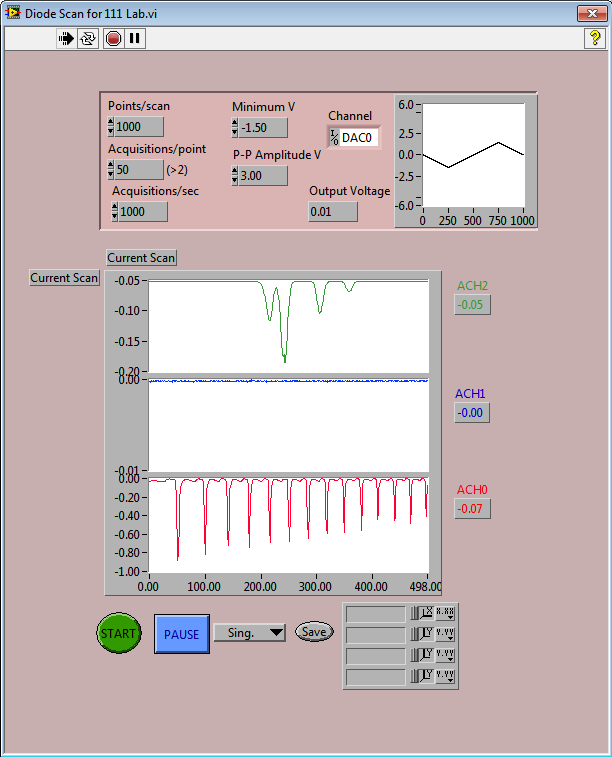
\includegraphics[width=0.5\linewidth]{images/Rb_doppler_spect.png}}
    \caption{The Diode Scan of the transmission spectrum of the F-P analyzer AI 0(ACH0) and laser-induced fluorescence AI 2(ACH2)}
    \label{fig:DiodeScanOfTransmissionSpectrum}
\end{figure}

On this picture, the AI 0 (ACH0) trace shows the transmission spectrum of the F-P analyzer. These are sometimes called ``frequency markers''; more negative signal means more transmitted light. The AI 1 (ACH1) input is not used and terminated (for the time being) and the AI 2 (ACH2) trace represents the laser-induced fluorescence spectrum.

\begin{itemize}
    \item Note: If you see some signals from one channel showing up in another, this means that there is ``cross-talk'' within the DAQ. To alleviate this problem, make sure that all signal amplitudes are under 1V. You can do this by reducing the gain of the amplifier, or closing down the aperture. AI 3 and AI 4 (the data from the polarimeter, PD-1 and PD-2) are another common source of cross talk. If you are not using these channels, you may want to leave them unplugged. They can distort the florescence spectrum beyond recognition. If you are using these channels and they are producing cross-talk try rotating the Polaroid film attenuator to reduce the amount of light hitting the diodes in the polarimeter.

\end{itemize}

\textbf{Q.} Explain the shape of the fluorescence spectrum. Which transitions correspond to the four fluorescence peaks? What determines their separation? What determines the width of a peak? The first article in the reprints shows this scan with the peaks labeled.

\begin{itemize}
    \item As a final step in this part of the lab, observe the fluorescence in real time. It is nice to record the signals electronically, but nothing compares to actually seeing the light as it happens! Adjust the Diode Scan program parameters, so the total scan time is several seconds (e.g. set 200 points per scan and 3 acquisitions per point), and the scanning is continuous. Using the night vision viewer, look at the side of the vapor cell as the laser is scanning.

\end{itemize}

\textbf{Q.} Describe what you see and explain these observations.

\subsection{Part 3: Doppler-free saturation spectroscopy}

In this part, you will obtain the saturated absorption spectrum of the D2-line, which is free from Doppler broadening. Doppler broadening arises because of thermal motion of radiating atoms, and often constitutes a major part of the total width of a spectral line. It is assumed here that you have read the relevant reprints and references and are familiar with the basic ideas on how this works. Preston and Weiman's article ``Doppler Free Saturated Absorption Spectroscopy: Laser Spectroscopy'' is a good place to start.

\begin{enumerate}
    \item The setup for this section is the same as in part 2. This time connect the photodiode PD-3 via a 1 M$\Omega$ PD Load Resistor to the A/I input of the SR830 lock-in amplifier (``A'' input should be selected). The reference frequency output ($f$) of the SR540 chopper controller should be connected to the REF IN input of the lock-in amplifier. The settings of the laser scan parameters, the chopper frequency, and the lock-in settings should all be consistent. You should optimize them for your particular experiment. Try these settings, and adjust them as necessary: lock-in time constant 30 ms, 12dB/Oct, AC coupling, sensitivity 100 mV, chopper frequency 400 Hz. Press ``Source'' on the right-hand-side of the lock-in until neither ``unlock'' or ``internal'' is lit up, the frequency display above the button will then read $\sim$400Hz (the chopper frequency). Scan the laser and simultaneously observe the Doppler-broadened laser-induced fluorescence and the Doppler-free saturation spectroscopy signals. Record the data and include the corresponding graphs in your report. Note that the widths and intensities of the saturation spectroscopy resonances depend on the powers of the laser beams and on their relative polarization. These parameters can be adjusted and optimized using combinations of Polaroid film sheets.

    \item Zoom in on each of the four transition groups, using procedure described below. Record your scans.

\end{enumerate}

\textbf{Procedure for Zooming In}

\textbf{Note:} As of 2013, with the new DAQ card the peaks can be zoomed in on with just software by adjusting the scanning parameters. Remember the laser has a linewidth of $\sim$100 kHz, how does this affect the useful range of ``zooming''?

\textbf{Old Procedure, No Need to Perform}

On the Diode scan program, set values for a scan which has an average voltage of 0 (e.g., Vmin = $-$1.5 and 3 Vpp), and press \textbf{Start} ONCE. (This will only set the values, but will not actually do a scan.) The reason for doing this is that even though the program is not scanning, it is still applying the average voltage to the ECU, which displays it.

Now do a regular (non-zoomed) scan over all the peaks and note the voltages at each of them. Now set LabView to do a scan, which has an average voltage of 0, but don't start the scan yet (only press \textbf{Start} once). Put in the 1:10 Divider (zoom resistor) and take another scan. What you've done is fool LabView into thinking that it is still sweeping near 0V with no offset, while the ECU is outputting a sweep around 0.904V, right where the peak is. The zoomed-in peak should now show up in your scan- if it is off a little, you can center it by adjusting the scan parameters in LabView. Repeat the process for the other three peaks.

\textbf{Q.} What is a \emph{cross-over resonance?} Do you see such resonances in your saturation spectroscopy scans? What determines the width of the saturation spectroscopy resonances?

3. In the analysis stage of your experiment, based on the data that you have recorded, you can determine the isotope shift of the transition and the hyperfine structure constants for both upper and lower states of each Rb isotope. The frequency markers that you have recorded are important for absolute calibration of your scans. It is up to you to work out the detailed analysis procedure. Include a comprehensive description in your report. Compare your results with the literature data. Reading up on isotope shifts and hyperfine structure will take lots of time. Don't hesitate to talk with the laboratory instructors when needed.

\subsection{Part 4: Optical polarimetry, nonlinear magneto optics}

In this part of the lab, you will use a laser polarimeter to investigate the resonant Faraday effect in Rb vapor. The Faraday effect is the rotation of the direction of polarization of linearly polarized light as it passes through a medium that has a magnetic field applied parallel to the direction of light propagation. In this experiment, we use light reflected from the beam splitter BS-4 (). This light first goes through two pieces of Polaroid film. These are used as a variable attenuator to adjust the light power (Both pieces of film are set on one mount. One piece is free to rotate and the other is fixed. Rotating the movable piece changes the amount of light that gets through.) Next, the beam goes through a precision prism polarizer and through a Rb vapor cell installed inside the magnetic shield. Note that we have in the laboratory equipment box several different cells with different isotopic compositions. The one inside the shield is likely to contain pure 85Rb, rather than an isotopic mixture. Verify the isotopic composition by comparing the spectra from this cell with those from the cell outside the shields, which contains a natural isotopic mixture. A magnet coil is installed inside the inner shield. This set-up is used to shield the lab magnetic field and to produce a well-controlled field along the axis of the chamber. Next, the light beam is split by a polarizing beam splitter (PBS) also known as polarimeter. The two resulting beams fall onto photodiodes (PD-1 and PD-2) which detect their power. To adjust the angle of the PBS mount, there is a course knob on the bottom of the dial, and a fine knob on the top. A good value to start with is to align the left number 260 with the 0 reference on the right. This might need adjusting to optimize signal, but it is a good starting point. This part is very delicate, ask for an instructor if you need help.

\textbf{Q.} Estimate the value \emph{of the residual magnetic} field at the vapor cell due to the Earth's and building's magnetic field. The article on magnetic shielding may be useful. Both layers of magnetic shielding are manufactured out of 0.04'' (1 mm) thick sheet of the CONETIC-AA alloy with a magnetic permeability $\mu = B/H \approx 10^5$. Calculate the calibration factor (in Gs/A) relating the value of the magnetic field produced by the coil and its current. Reproduce these estimates and calculations in your report. \textbf{Hint:} the presence of the magnetic shield actually affects the field inside the coil.

To measure rotation of the plane of polarization in a sample, it is placed between two polarizers as shown in Figure \ref{fig:SchematicOfBalancedPolarimeter}, in what is called a balanced polarimeter. The Polarizer and Polarized Beam Splitter (PBS) have their transmission axes oriented at 45 degrees to one another.

\begin{figure}[h]
    \centering
    \href{http://experimentationlab.berkeley.edu/sites/default/files/images/MNOimage008.gif}{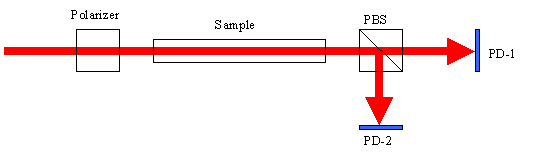
\includegraphics[width=0.5\linewidth]{images/MNOimage008.png}}
    \caption{Schematic of a balanced polarimeter}
    \label{fig:SchematicOfBalancedPolarimeter}
\end{figure}

Consider the two light beams emerging from the PBS and falling onto the photodiodes PD-1 and PD-2. The transmitted powers of these beams for an ideal lossless PBS is:
\begin{align*}
    P_1 &= P_0\cos^2{\theta} \\
    P_2 &= P_0\sin^2{\theta} \\
    P_0 &= P_1+P_2
\end{align*}
where $P_0$ is the light power entering the PBS, and $\theta$ is the angle between the polarization axis of the light and the PBS axis.

When the angle between the Polarizer and the PBS transmission axes is set to $\pi/4$, we have $\theta = \frac{\pi}{4}+\delta $, where $ \delta $ is the angle of polarization rotation in the sample. Using trigonometric formulas and assuming that $\delta \ll 1$, we find that
\begin{gather*}
    \cos^2{\theta} = \frac{1+\cos{2\theta}}{2}, \quad \sin^2{\theta} = \frac{1-\cos{2\theta}}{2}, \quad \cos{\frac{\pi}{2} + 2\delta} \approx -2\delta \\
    P_1 - P_2 \approx 2\times P_0 \times \delta = 2 \times (P_1 + P_2) \times \delta
\end{gather*}
The optical rotation in the sample is then
\[
    \delta = \frac{P_1 - P_2}{2(P_1 + P_2)}
\]
This equation is programmed into LabView (``B-field scan for 111 lab.vi'').

\textbf{Q.} How would this result change if along with polarization rotation in the sample there were circular dichroism - unequal absorption for the right- and left-circular polarizations? Consider small rotation and dichroism, so the two effects can be treated independently.

\begin{itemize}
    \item Direct the laser beam from BS-4 into the magnetic shield assembly and the balanced polarimeter (see Figure \ref{fig:BlockDiagramOfElectricalConnections}). Make sure that the beam is centered both on the input and the output of each element. It should be possible to achieve this by adjusting the beam splitter BS-4 and the relevant optical and magnetic shield assembly mounts.

\end{itemize}

\subsubsection{Procedure for the Optical Rotation Equipment}

\begin{enumerate}
    \item Connect PD-6 to AI2 through the load resistor in the following way: the cable labeled ``from PD-6'' needs to take the place of ``from PD-5'' on input of the load resistor. ``Cable 7'' needs to take the place of ``Cable 5'' on the output of the load resistor. AO 0 from the Breakout Box should be connected to the back of the ECU via cable 1.

    \item Run a diode scan but this time increase the points/scan and decrease the acquisitions/second to make the scan go slower. Then stop the program when the laser frequency is centered on the 85Rb Fg=3 level (the most prominent ground state level) by clicking the stop button below the charts. This ensures that the rubidium sample inside the magnetic field chamber is fluorescing. To do this efficiently, click stop while the signal is on its way down. Check that the chamber is fluorescing using the Night Vision Viewer. If you see no glow or only a faint glow, try adjusting the offset button \emph{slightly}to strengthen the glow. Be careful not to turn the offset button too far, you should not have to turn it more than about half a rotation. Then make sure you completely stop the program by clicking the other stop button in the upper left hand corner.

    \item Next, connect the two outputs of the balance polarimeter (PD-1 and PD-2) to channel 1 and 2 on an oscilloscope and set the scope to add the channels together. The value of the signal should be around -850 mV or below. If this is the case, you will not have to make any adjustments to the optical equipment on the table. If the signal is -700 mV or above, you may need to make some adjustments. PROCEED WITH CAUTION--you do not want to accidentally make the alignment worse, so only make slight adjustments and keep track of everything. Try adjusting the beam splitter, and the orientation and height of the polarimeter so that the voltage displayed on the scope is as negative as possible (negative voltage means light is hitting the diode).

    \item Now, connect PD-1 to data acquisition input AI 3 via cable 6 and PD-2 to AI 4 via cable 8 using the 100 K$\Omega$ PD Load Resistance boxes. Keep the AO 0 connected to the ECU input via cable 1. Connect the AO 1 output to the Input 1 of the COIL DRIVER via cable 3. The magnetic coil has a resistance of 3.9$\Omega$, and the I-V curve is the following:
    \begin{figure}[h]
        \centering
        \href{http://experimentationlab.berkeley.edu/sites/default/files/images/Voltagecurrentplot.jpg}{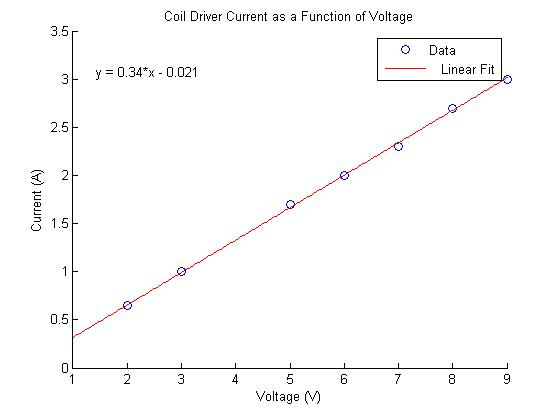
\includegraphics[width=0.5\linewidth]{images/Voltagecurrentplot.jpg}}
        \caption{Plot showing the linearity of the coil}
        \label{fig:Voltagecurrentplot}
    \end{figure}
    
    As one can see, the current in the coil is linear with its input voltage. The Output 1 of the Coil Driver goes to the magnetic coil. The computer will use the AO 1 output to scan the magnetic coil from -8V to +8V. The current source produces an output current in the approximate range -3 to +3A, proportional to the voltage at its input. \textbf{The input cable to the coil driver power supply must be plugged in the reverse leads to operate correctly. It should be like this already, but double check.} It will be necessary for you to obtain current calibration, i.e., to figure out precisely which current corresponds to a given AO 1 voltage. Hook up a multimeter to the .1$\Omega$ resistor (it is a gold cylinder) located to the right of the coil driver. The DMM should already be connected to measure the voltage across the resistor, but ensure the connections are made properly. \textbf{It registers 100mV for every Amp driven through the coil.}

    \item Magnetic field control in this experiment is accomplished with a LabView VI program ``B field Scan for 111 lab''. This program is nearly identical with the ``Diode scan for 111 lab.vi'' program. We use both programs sequentially to tune the laser to the frequency at which we wish to take a B-field scan and to scan the magnetic field. When all necessary connections and beam alignment have been done, use the Night Vision Viewer to verify that the laser is still fluorescing within the Rb glass cell. If it is not glowing, go back to Step 2 and restart the diode scan. If it is glowing faintly, try slightly adjust the offset.
    
    \begin{itemize}
        \item When there is a strong glow, start the ``B field scan for 111 lab.vi'' (you must ensure that the Diode Scan program is completely stopped, pressing stop in the upper left hand corner, before scanning the B field. If this is not done, you will see nothing when scanning the B field) and take a single scan across the atomic resonance encompassing all four line groups. The settings should be 1000 points/scan, 15 Acquisitions/point, 500 Acquisitions/second, $-$5.00 V Min Voltage, and 10.00 V P-P Amp Voltage. It should look something like Figure \ref{fig:BFieldScan}.
    
    \end{itemize}
    
    \begin{figure}[h]
        \centering
        \href{http://experimentationlab.berkeley.edu/sites/default/files/images/MNOimage020.jpg}{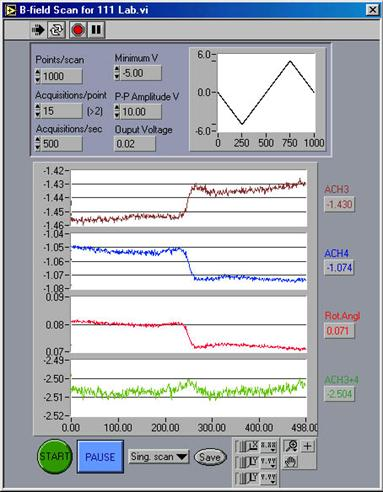
\includegraphics[width=0.5\linewidth]{images/MNOimage020.jpg}}
        \caption{The B-Field Scan}
        \label{fig:BFieldScan}
    \end{figure}
    
    \item Before proceeding further, you have to balance the polarimeter, i.e. make sure that the value of the ``optical rotation angle'' that you see when the laser is not on resonance is close to zero. Run the Diode Scan program and pause the laser frequency far from any peaks. The pause button text should change to \textbf{Resume} indicating that a repeated click on the button will resume the frequency scan. Then run the ``B-field scan for 111 lab.vi'' in continuous mode. While the scan is running, adjust the angle of the PBS mount to zero the apparent optical rotation angle. Make note of what numbers were lined up before you make any changes--there is a good chance it is already set close to the correct values. Try setting the number 252 on the left to line up with the number 0 on the right.
    
    \item You are now ready to take Faraday effect data. Decide at which frequency point you would like to study the B-dependence of the Faraday rotation. A good first choice is the center of the F = 3 $\rightarrow$ F' peak for 85Rb. Run the Diode Scan again to scan the laser frequency and stop the scan on this peak. Then be sure to stop the Diode Scan program, and open up and run the ``B-field scan for 111 lab.vi''. The settings should be 1000 points/scan, 15 Acquisitions/point, 500 Acquisitions/second, -5.00 V Min Voltage, and 10.00 V P-P Amp Voltage. The signals should look like Figure \ref{fig:BFieldScan}. This allows you to set the magnetic field (i.e. AO 1) scan parameters and display raw signal from one of the photodiodes (PD-1, or PD-2). The optical rotation angle determined as discussed above, and the sum of signals of photodiodes (PD-1 and PD-2) is a measure of power of the laser beam after the sample.
    
    \item Here is the second major assignment in this lab: investigate the magnetic field dependence of NLFR; demonstrate the existence of three contributions to NLFR (see \hyperref[sec:BeforeFirstDay]{Prerequisite Reading Materials} for detailed discussion): ``hole burning'', ``transit effect'', and the ``wall-collision induced effect''. \textbf{IMPORTANT: The rubidium cell inside the magnetic shield is not coated so it is impossible to see the ``wall-collision induced effect''.} If possible, determine the width of the peaks in the magnetic field dependence of the rotation corresponding to each of these mechanisms. How do these values compare with what might be expected? When you zoom onto the narrowest features in the magnetic field dependence of the optical rotation, you should not use the current source since because of its high gain, the resolution is limited by the discreteness of the computer DAC. Instead, connect the DAC (i.e. the signal used as input to the current source) to the magnetic coils through a 2.5 k$\Omega$ resistor (provided in a small blue box with two BNC connectors). This converts the DAC into a current source with I = VDAC/2.5 k$\Omega$, where we neglect the small resistance of the magnetic coil.
    
    \begin{itemize}
        \item Warning! Make sure that there is no current running through the coils when you break the circuit in order to add the resistor. When you break a circuit that contains an inductor (i.e. the magnetic coils) all the power contained in the inductor is dumped in the backward direction through the circuit, which can blow out the power supply.
    
    \end{itemize}
    
    \textbf{Q.} What is the magnitude of the linear Faraday rotation (the Macaluso-Corbino effect)? Is it observed in these experiments?

\end{enumerate}

\begin{itemize}
    \item Last day of the experiment please fill out the \href{\ExperimentEvaluation}{\textbf{Experiment Evaluation}}

\end{itemize}

\end{document}
